\documentclass{article}
\usepackage{tikz}
\usetikzlibrary{automata, positioning, arrows}
\usepackage[margin=1cm]{geometry}
\usepackage{caption}

\begin{document}
\section*{Zadanie 1}
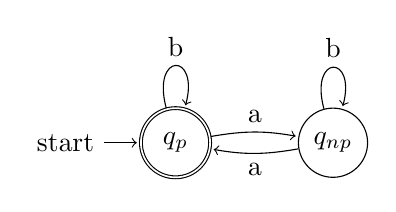
\begin{tikzpicture}[shorten >=1pt,node distance=2cm,on grid,auto]

   \node[state,initial,accepting] (q_p)   {$q_p$}; 
   \node[state] (q_np) [right=of q_p] {$q_{np}$}; 

   \path[->]
   (q_p) edge [loop above] node {b} ()
         edge [bend left=10] node {a} (q_np)
   (q_np) edge [loop above] node {b} ()
         edge [bend left=10] node {a} (q_p);

    
\end{tikzpicture}

\section*{Zadanie 2}
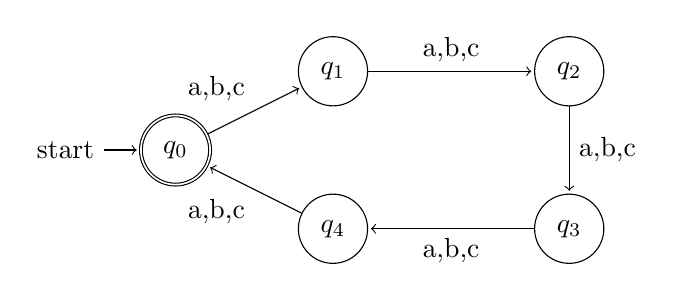
\begin{tikzpicture}[shorten >=1pt,node distance=2cm,on grid,auto]

   \node[state,initial,accepting] (q_0)   {$q_0$}; 
   \node[state] (q_1) [above right=1cm and 2cm of q_0] {$q_1$}; 
   \node[state] (q_2) [right=3cm of q_1,] {$q_2$}; 
   \node[state] (q_4) [below right=1cm and 2cm of q_0] {$q_4$};
   \node[state] (q_3) [right=3cm of q_4] {$q_3$};

   \path[->]
    (q_0) edge node {a,b,c} (q_1)
    (q_1) edge node {a,b,c} (q_2)
    (q_2) edge node {a,b,c} (q_3)
    (q_3) edge node {a,b,c} (q_4)
    (q_4) edge node {a,b,c} (q_0);
    
\end{tikzpicture}

\section*{Zadanie 3}
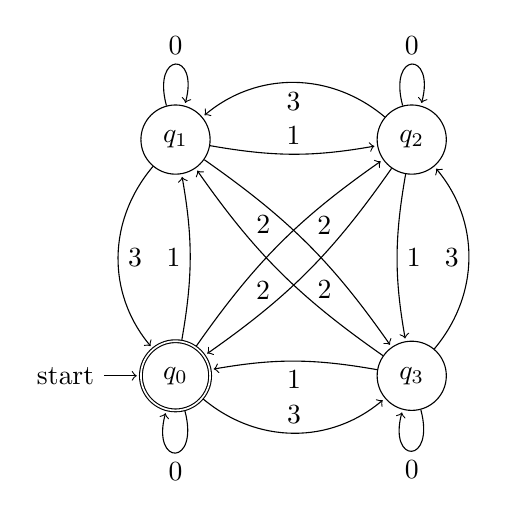
\begin{tikzpicture}[shorten >=1pt,node distance=2cm,on grid,auto]

   \node[state,initial,accepting] (q_0)   {$q_0$}; 
   \node[state] (q_1) [above=3cm of q_0] {$q_1$}; 
   \node[state] (q_2) [right=3cm of q_1,] {$q_2$}; 
   \node[state] (q_3) [below=3cm of q_2] {$q_3$};

   \path[->]
   (q_0) edge [loop below] node {0} ()
         edge [bend right=10] node {1} (q_1)
         edge [bend left=10] node {2} (q_2)
         edge [bend right=40] node {3} (q_3)
   (q_1) edge [loop above] node {0} ()
         edge [bend right=10] node {1} (q_2)
         edge [bend left=10] node {2} (q_3)
         edge [bend right=40] node {3} (q_0)
   (q_2) edge [loop above] node {0} ()
         edge [bend right=10] node {1} (q_3)
         edge [bend left=10] node {2} (q_0)
         edge [bend right=40] node {3} (q_1)
   (q_3) edge [loop below] node {0} ()
         edge [bend right=10] node {1} (q_0)
         edge [bend left=10] node {2} (q_1)
         edge [bend right=40] node {3} (q_2);
    

\end{tikzpicture}

\section*{Zadanie 4}
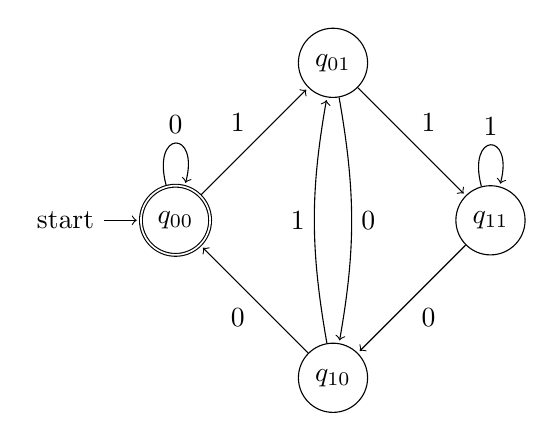
\begin{tikzpicture}[shorten >=1pt,node distance=2cm,on grid,auto]

   \node[state,initial,accepting] (q_00)   {$q_{00}$}; 
   \node[state] (q_01) [above right=2cm and 2cm of q_00] {$q_{01}$}; 
   \node[state] (q_11) [right= 4cm of q_00,] {$q_{11}$}; 
   \node[state] (q_10) [below right=2cm and 2cm of q_00] {$q_{10}$};

   \path[->]
   (q_00) edge [loop above] node {0} ()
          edge node {1} (q_01)
   (q_01) edge node {1} (q_11)
          edge [bend left=10] node {0} (q_10)
   (q_11) edge [loop above] node {1} ()
          edge node {0} (q_10)
   (q_10) edge [bend left=10] node{1} (q_01)
          edge node {0} (q_00);
    
\end{tikzpicture}

\section*{Zadanie 5}
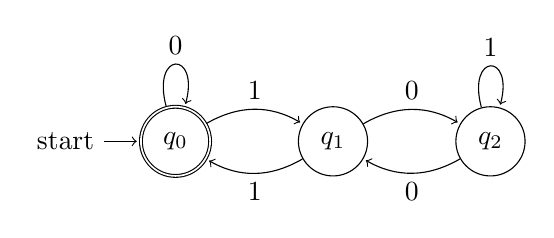
\begin{tikzpicture}[shorten >=1pt,node distance=2cm,on grid,auto]

   \node[state,initial,accepting] (q_0)   {$q_0$}; 
   \node[state] (q_1) [right=of q_0] {$q_1$}; 
   \node[state] (q_2) [right=of q_1] {$q_2$}; 
    
    \path[->] 
    (q_0) edge [bend left] node {1} (q_1)
          edge [loop above] node {0} ()
    (q_1) edge [bend left] node  {0} (q_2)
          edge [bend left] node {1} (q_0)
    (q_2) edge [bend left] node {0} (q_1)
          edge [loop above] node {1} ();
\end{tikzpicture}
\end{document}